\subsection{OpenMP benchmark}\label{subsec:openmp}

Figure \ref{fig:scaling-openmp} reports the parallel scaling analysis performed with OpenMP directives-based paradigm. This benchmark has been done on a \emph{dual Intel(R) Xeon(R) CPU X5650} exacores workstation for a total of 12 physical cores, coupled with 24GB of RAM. The codes (with and without FOODIE) have been compiled by means of the GNU gfortran compiler v5.2.0 with \emph{-O2 -fopenmp} compilation flags.

The Euler conservation laws are integrated for 10 time steps by means of the TVD RK(5,4) solver: the measured CPU time used for computing the scaling efficiencies is the average of the 10 integrations, thus representing the mean CPU time for computing one time step integration.

For the strong scaling, the benchmark has been conducted with 100000 finite volumes. Figure \ref{fig:strong-scaling-openmp} summarizes the strong scaling analysis: it shows that FOODIE-based code scales similarly to the baseline code without FOODIE.

For the weak scaling the minimum size if 10000 finite volumes and the size is scaled linearly with the OpenMP threads, thus $N_{12} = 120000$ cells. Figure \ref{fig:weak-scaling-openmp} summarizes the weak scaling analysis and it essentially confirms that FOODIE-based code scales similarly to the baseline code without FOODIE.

Both strong and weak scaling analysis point out that for the computing architecture considered the parallel scaling is reasonable up to 8 cores: using 12 cores the measured efficiencies become unsatisfactory, reducing below the 50\%.
\begin{figure}[!ht]
  \centering
  \begin{subfigure}[b]{0.95\textwidth}
    \centering
    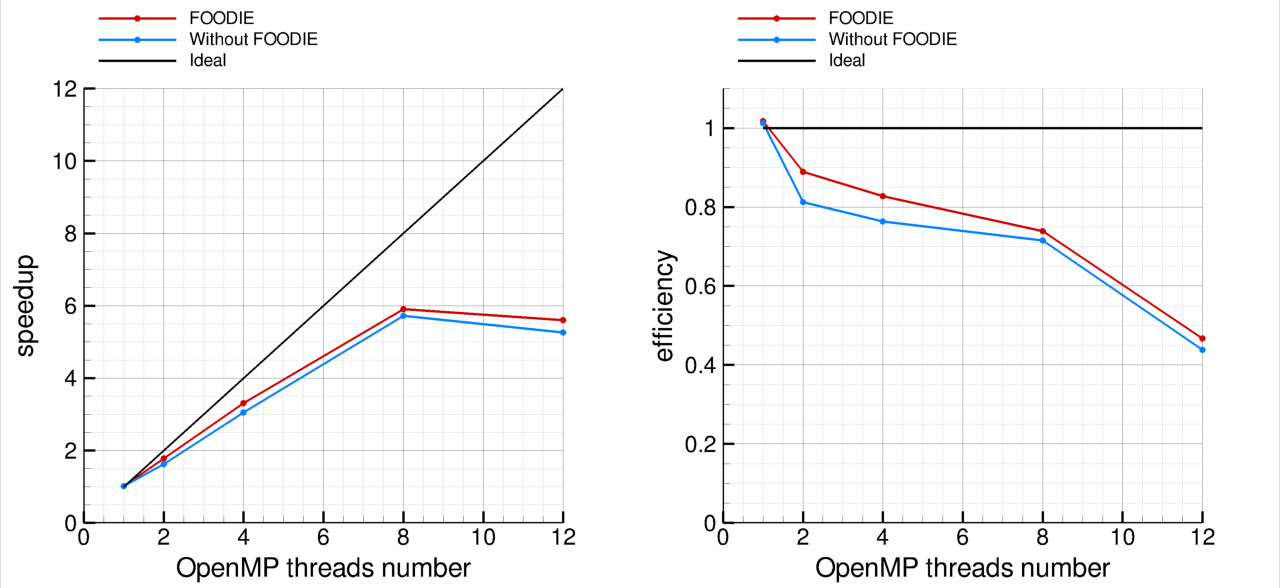
\includegraphics[width=1.00\textwidth]{openmp_benchmark/euler-1D-openmp/strong-scaling-comparison.png}
    \caption{Strong scaling, number of cells 100000}\label{fig:strong-scaling-openmp}
  \end{subfigure}\\
  \begin{subfigure}[b]{0.95\textwidth}
    \centering
    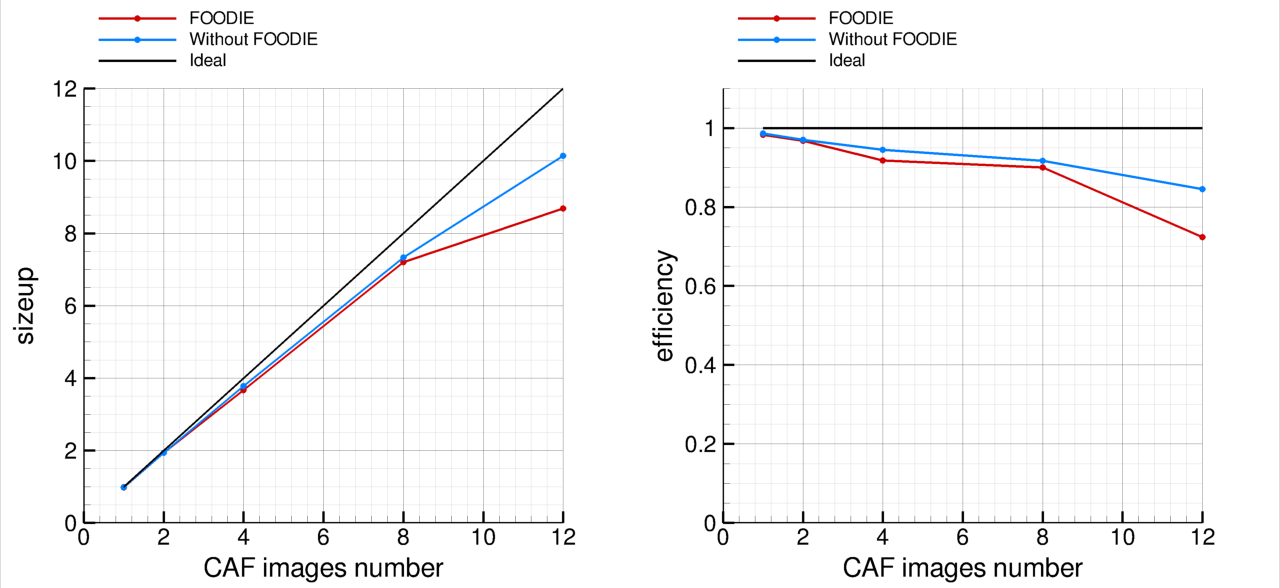
\includegraphics[width=1.00\textwidth]{openmp_benchmark/euler-1D-openmp/weak-scaling-comparison.png}
    \caption{Weak scaling, minimum number of cells 10000}\label{fig:weak-scaling-openmp}
  \end{subfigure}\\
  \caption{Scaling efficiency with OpenMP programming model}\label{fig:scaling-openmp}
\end{figure}

